\chapter[Proton and Antiproton DCA Distributions]{Proton and Antiproton DCA Distributions - only STAR NOTE}\label{appendix:DCA_proton}
\begin{figure}[h!]
	\centering
	\begin{subfigure}{.45\textwidth}
		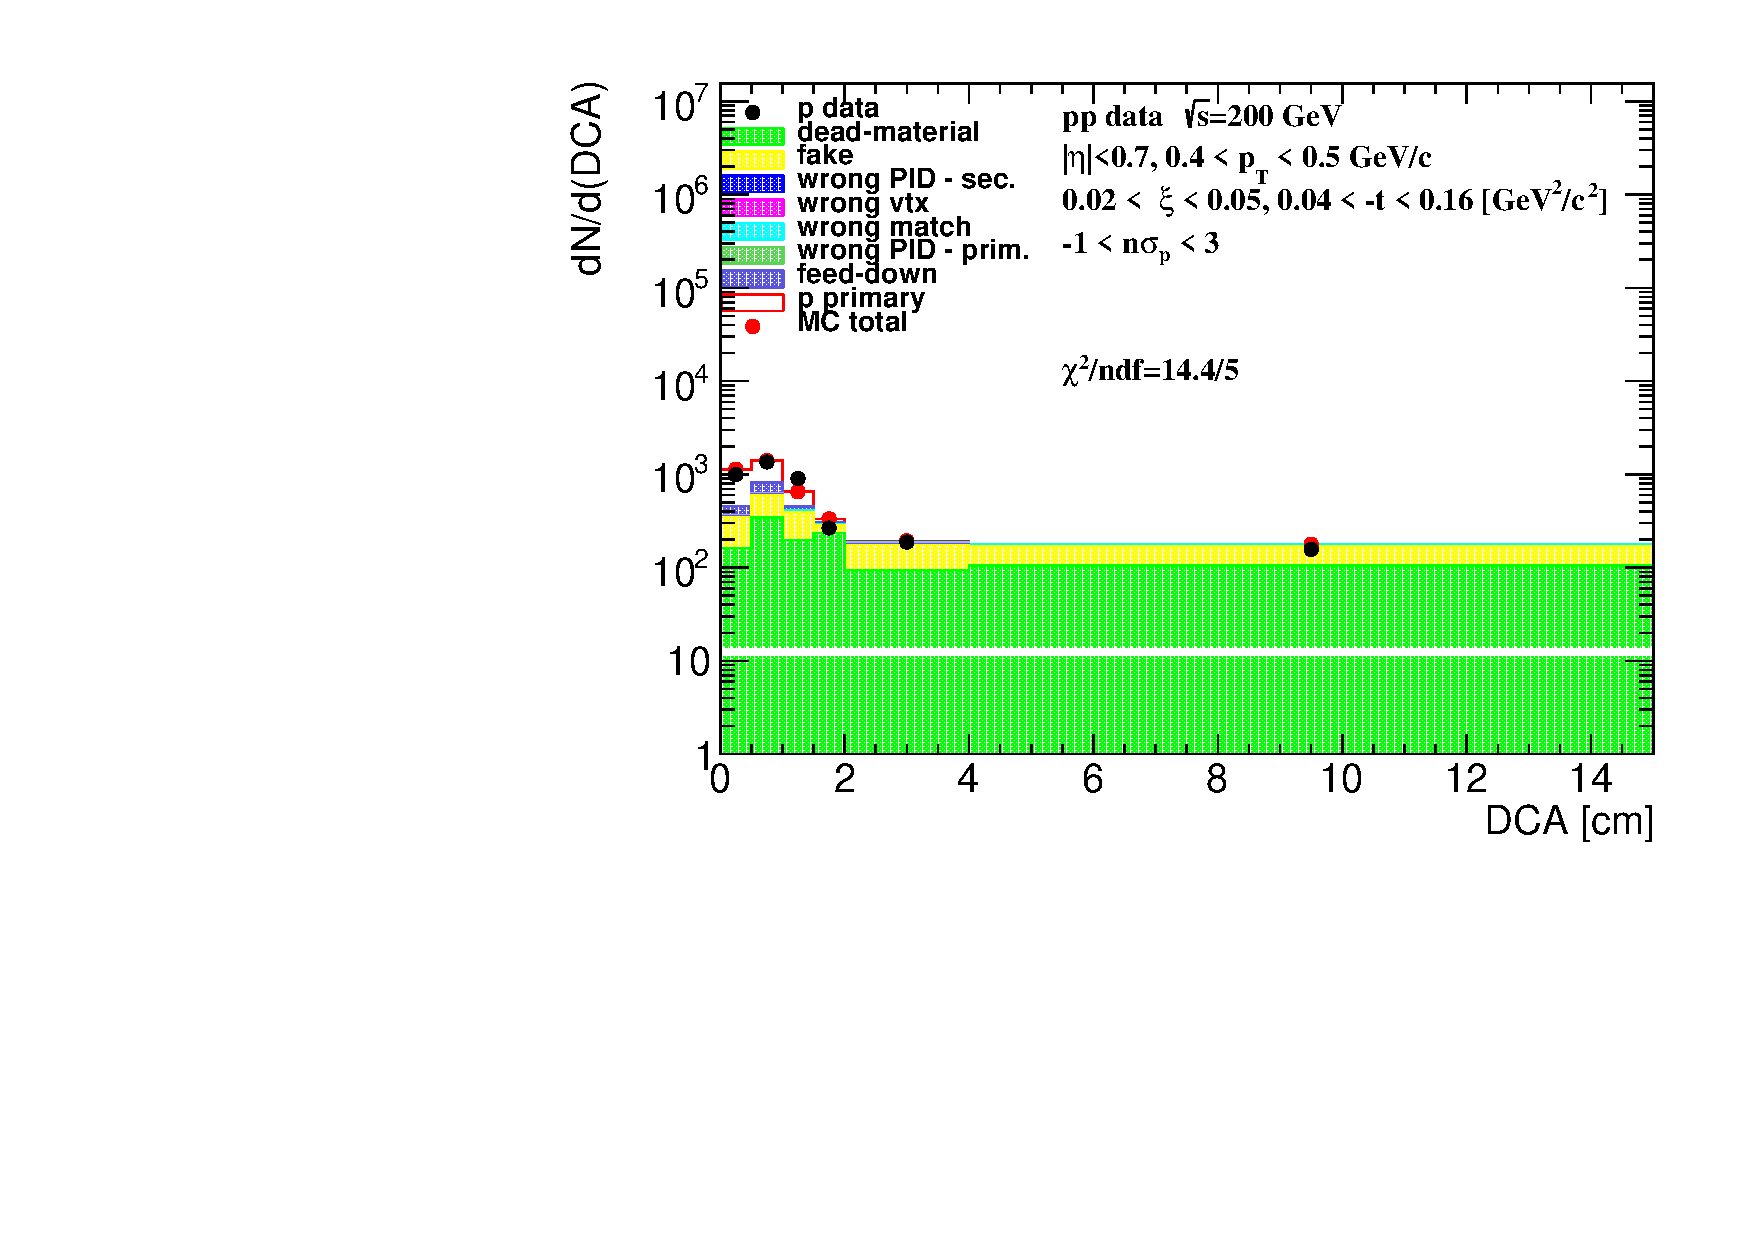
\includegraphics[width=\linewidth, page=1]{chapters/chrgSTAR/img/DCAproton/background_p_0.pdf}
	\end{subfigure}
	\begin{subfigure}{.45\textwidth}
		\includegraphics[width=\linewidth, page=2]{chapters/chrgSTAR/img/DCAproton/background_p_0.pdf}
	\end{subfigure}
	\begin{subfigure}{.45\textwidth}
		\includegraphics[width=\linewidth, page=5]{chapters/chrgSTAR/img/DCAproton/background_p_0.pdf}
	\end{subfigure}
	\begin{subfigure}{.45\textwidth}
		\includegraphics[width=\linewidth, page=6]{chapters/chrgSTAR/img/DCAproton/background_p_0.pdf}
	\end{subfigure}
	\begin{subfigure}{.45\textwidth}
		\includegraphics[width=\linewidth, page=9]{chapters/chrgSTAR/img/DCAproton/background_p_0.pdf}
	\end{subfigure}
	\begin{subfigure}{.45\textwidth}
		\includegraphics[width=\linewidth, page=10]{chapters/chrgSTAR/img/DCAproton/background_p_0.pdf}
	\end{subfigure}
	\begin{subfigure}{.45\textwidth}
		\includegraphics[width=\linewidth, page=13]{chapters/chrgSTAR/img/DCAproton/background_p_0.pdf}
	\end{subfigure}
	\begin{subfigure}{.45\textwidth}
		\includegraphics[width=\linewidth, page=14]{chapters/chrgSTAR/img/DCAproton/background_p_0.pdf}
	\end{subfigure}
	\caption{Distributions of DCA for protons in SD interactions with $0.02 < \xi<0.05$ and loose selection.}
	\label{fig:dca_proton_0}
\end{figure}
\begin{figure}[h!]
	\centering
	\begin{subfigure}{.45\textwidth}
		\includegraphics[width=\linewidth, page=3]{chapters/chrgSTAR/img/DCAproton/background_p_0.pdf}
	\end{subfigure}
	\begin{subfigure}{.45\textwidth}
		\includegraphics[width=\linewidth, page=4]{chapters/chrgSTAR/img/DCAproton/background_p_0.pdf}
	\end{subfigure}
	\begin{subfigure}{.45\textwidth}
		\includegraphics[width=\linewidth, page=7]{chapters/chrgSTAR/img/DCAproton/background_p_0.pdf}
	\end{subfigure}
	\begin{subfigure}{.45\textwidth}
		\includegraphics[width=\linewidth, page=8]{chapters/chrgSTAR/img/DCAproton/background_p_0.pdf}
	\end{subfigure}
	\begin{subfigure}{.45\textwidth}
		\includegraphics[width=\linewidth, page=11]{chapters/chrgSTAR/img/DCAproton/background_p_0.pdf}
	\end{subfigure}
	\begin{subfigure}{.45\textwidth}
		\includegraphics[width=\linewidth, page=12]{chapters/chrgSTAR/img/DCAproton/background_p_0.pdf}
	\end{subfigure}
	\begin{subfigure}{.45\textwidth}
		\includegraphics[width=\linewidth, page=15]{chapters/chrgSTAR/img/DCAproton/background_p_0.pdf}
	\end{subfigure}
	\begin{subfigure}{.45\textwidth}
		\includegraphics[width=\linewidth, page=16]{chapters/chrgSTAR/img/DCAproton/background_p_0.pdf}
	\end{subfigure}
	\caption{Distributions of DCA for protons in SD interactions with $0.02 < \xi<0.05$ and normal selection.}
	\label{fig:dca_proton_0t}
\end{figure}
\begin{figure}[h!]
	\centering
	\begin{subfigure}{.45\textwidth}
		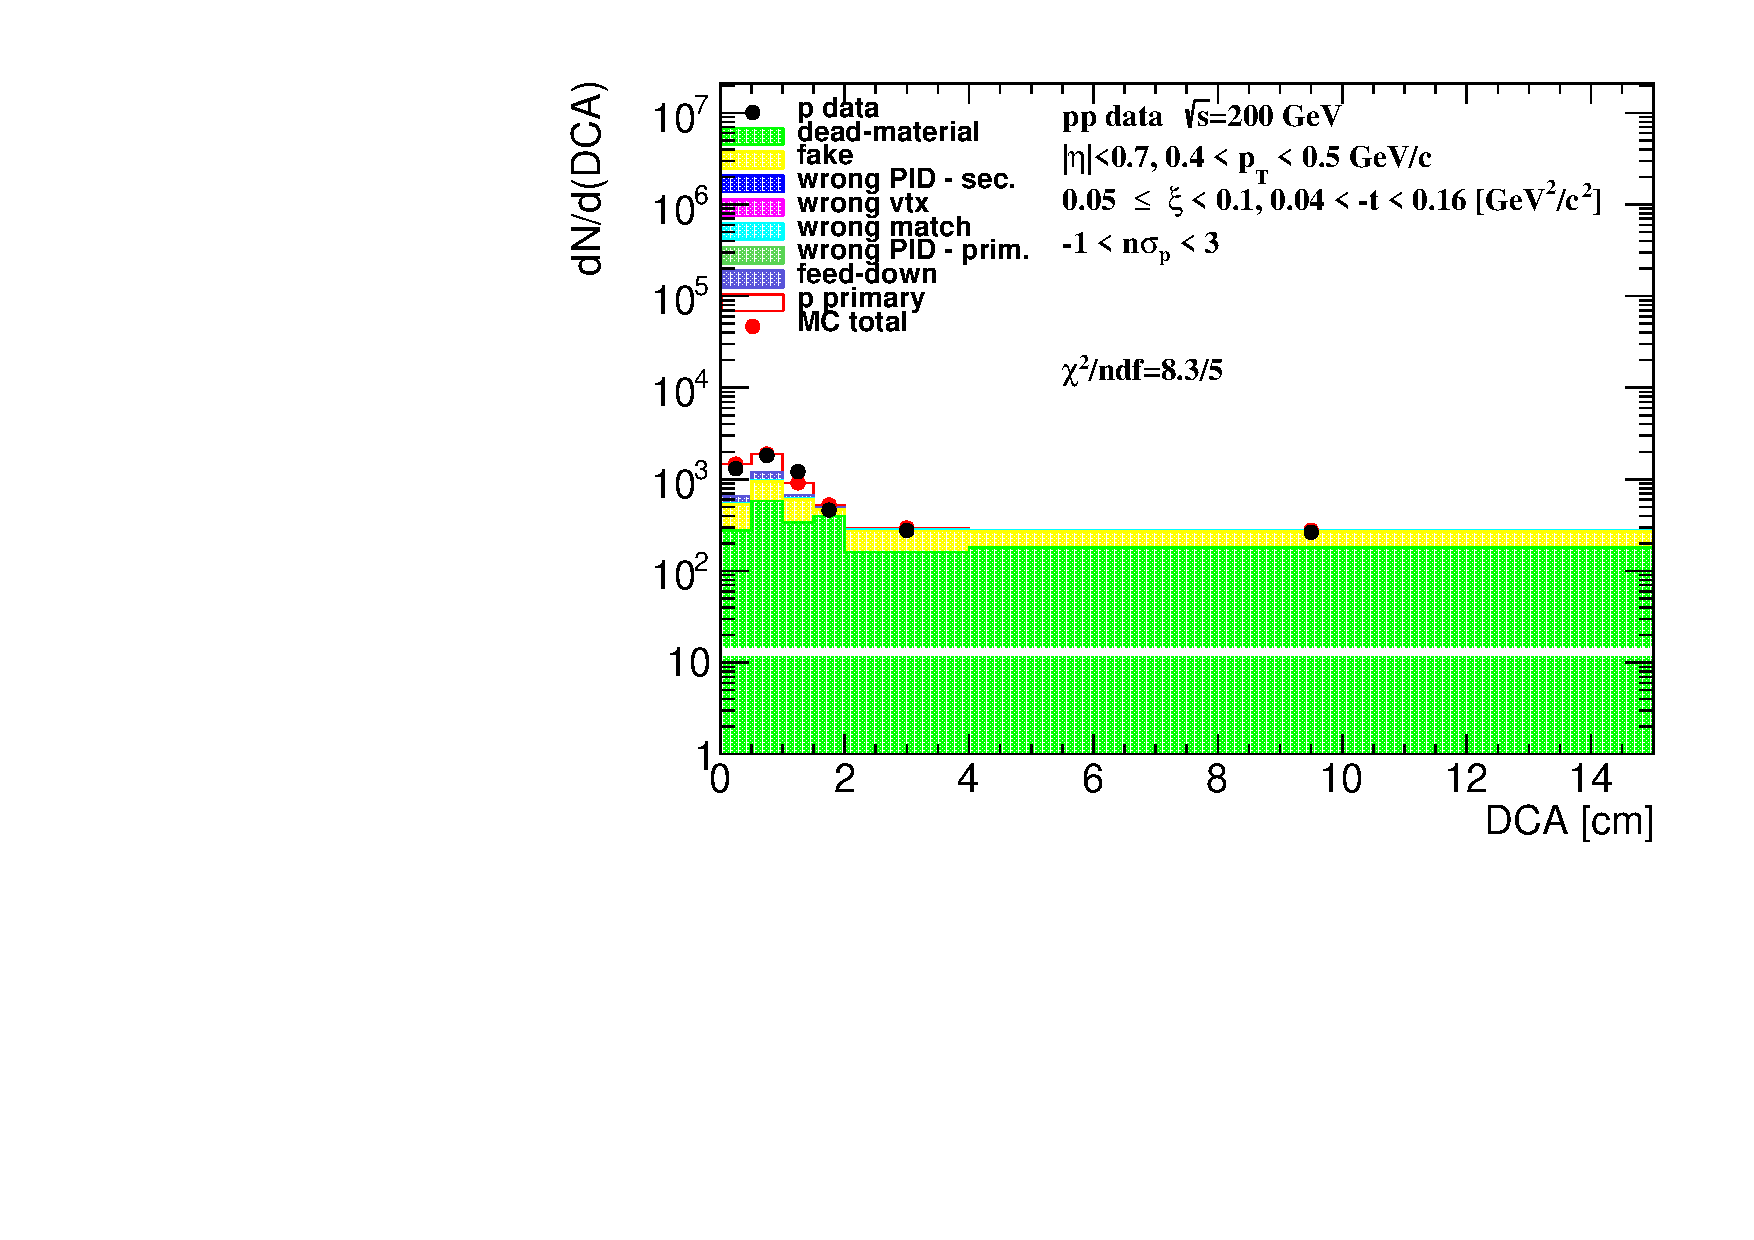
\includegraphics[width=\linewidth, page=1]{chapters/chrgSTAR/img/DCAproton/background_p_1.pdf}
	\end{subfigure}
	\begin{subfigure}{.45\textwidth}
		\includegraphics[width=\linewidth, page=2]{chapters/chrgSTAR/img/DCAproton/background_p_1.pdf}
	\end{subfigure}
	\begin{subfigure}{.45\textwidth}
		\includegraphics[width=\linewidth, page=5]{chapters/chrgSTAR/img/DCAproton/background_p_1.pdf}
	\end{subfigure}
	\begin{subfigure}{.45\textwidth}
		\includegraphics[width=\linewidth, page=6]{chapters/chrgSTAR/img/DCAproton/background_p_1.pdf}
	\end{subfigure}
	\begin{subfigure}{.45\textwidth}
		\includegraphics[width=\linewidth, page=9]{chapters/chrgSTAR/img/DCAproton/background_p_1.pdf}
	\end{subfigure}
	\begin{subfigure}{.45\textwidth}
		\includegraphics[width=\linewidth, page=10]{chapters/chrgSTAR/img/DCAproton/background_p_1.pdf}
	\end{subfigure}
	\begin{subfigure}{.45\textwidth}
		\includegraphics[width=\linewidth, page=13]{chapters/chrgSTAR/img/DCAproton/background_p_1.pdf}
	\end{subfigure}
	\begin{subfigure}{.45\textwidth}
		\includegraphics[width=\linewidth, page=14]{chapters/chrgSTAR/img/DCAproton/background_p_1.pdf}
	\end{subfigure}
	\caption{Distributions of DCA for protons in SD interactions with $0.05 < \xi<0.1$ and loose selection.}
	\label{fig:dca_proton_1}
\end{figure}
\begin{figure}[h!]
	\centering
	\begin{subfigure}{.45\textwidth}
		\includegraphics[width=\linewidth, page=3]{chapters/chrgSTAR/img/DCAproton/background_p_1.pdf}
	\end{subfigure}
	\begin{subfigure}{.45\textwidth}
		\includegraphics[width=\linewidth, page=4]{chapters/chrgSTAR/img/DCAproton/background_p_1.pdf}
	\end{subfigure}
	\begin{subfigure}{.45\textwidth}
		\includegraphics[width=\linewidth, page=7]{chapters/chrgSTAR/img/DCAproton/background_p_1.pdf}
	\end{subfigure}
	\begin{subfigure}{.45\textwidth}
		\includegraphics[width=\linewidth, page=8]{chapters/chrgSTAR/img/DCAproton/background_p_1.pdf}
	\end{subfigure}
	\begin{subfigure}{.45\textwidth}
		\includegraphics[width=\linewidth, page=11]{chapters/chrgSTAR/img/DCAproton/background_p_1.pdf}
	\end{subfigure}
	\begin{subfigure}{.45\textwidth}
		\includegraphics[width=\linewidth, page=12]{chapters/chrgSTAR/img/DCAproton/background_p_1.pdf}
	\end{subfigure}
	\begin{subfigure}{.45\textwidth}
		\includegraphics[width=\linewidth, page=15]{chapters/chrgSTAR/img/DCAproton/background_p_1.pdf}
	\end{subfigure}
	\begin{subfigure}{.45\textwidth}
		\includegraphics[width=\linewidth, page=16]{chapters/chrgSTAR/img/DCAproton/background_p_1.pdf}
	\end{subfigure}
	\caption{Distributions of DCA for protons in SD interactions with $0.05< \xi<0.1$ and normal selection.}
	\label{fig:dca_proton_1t}
\end{figure}
\begin{figure}[h!]
	\centering
	\begin{subfigure}{.45\textwidth}
		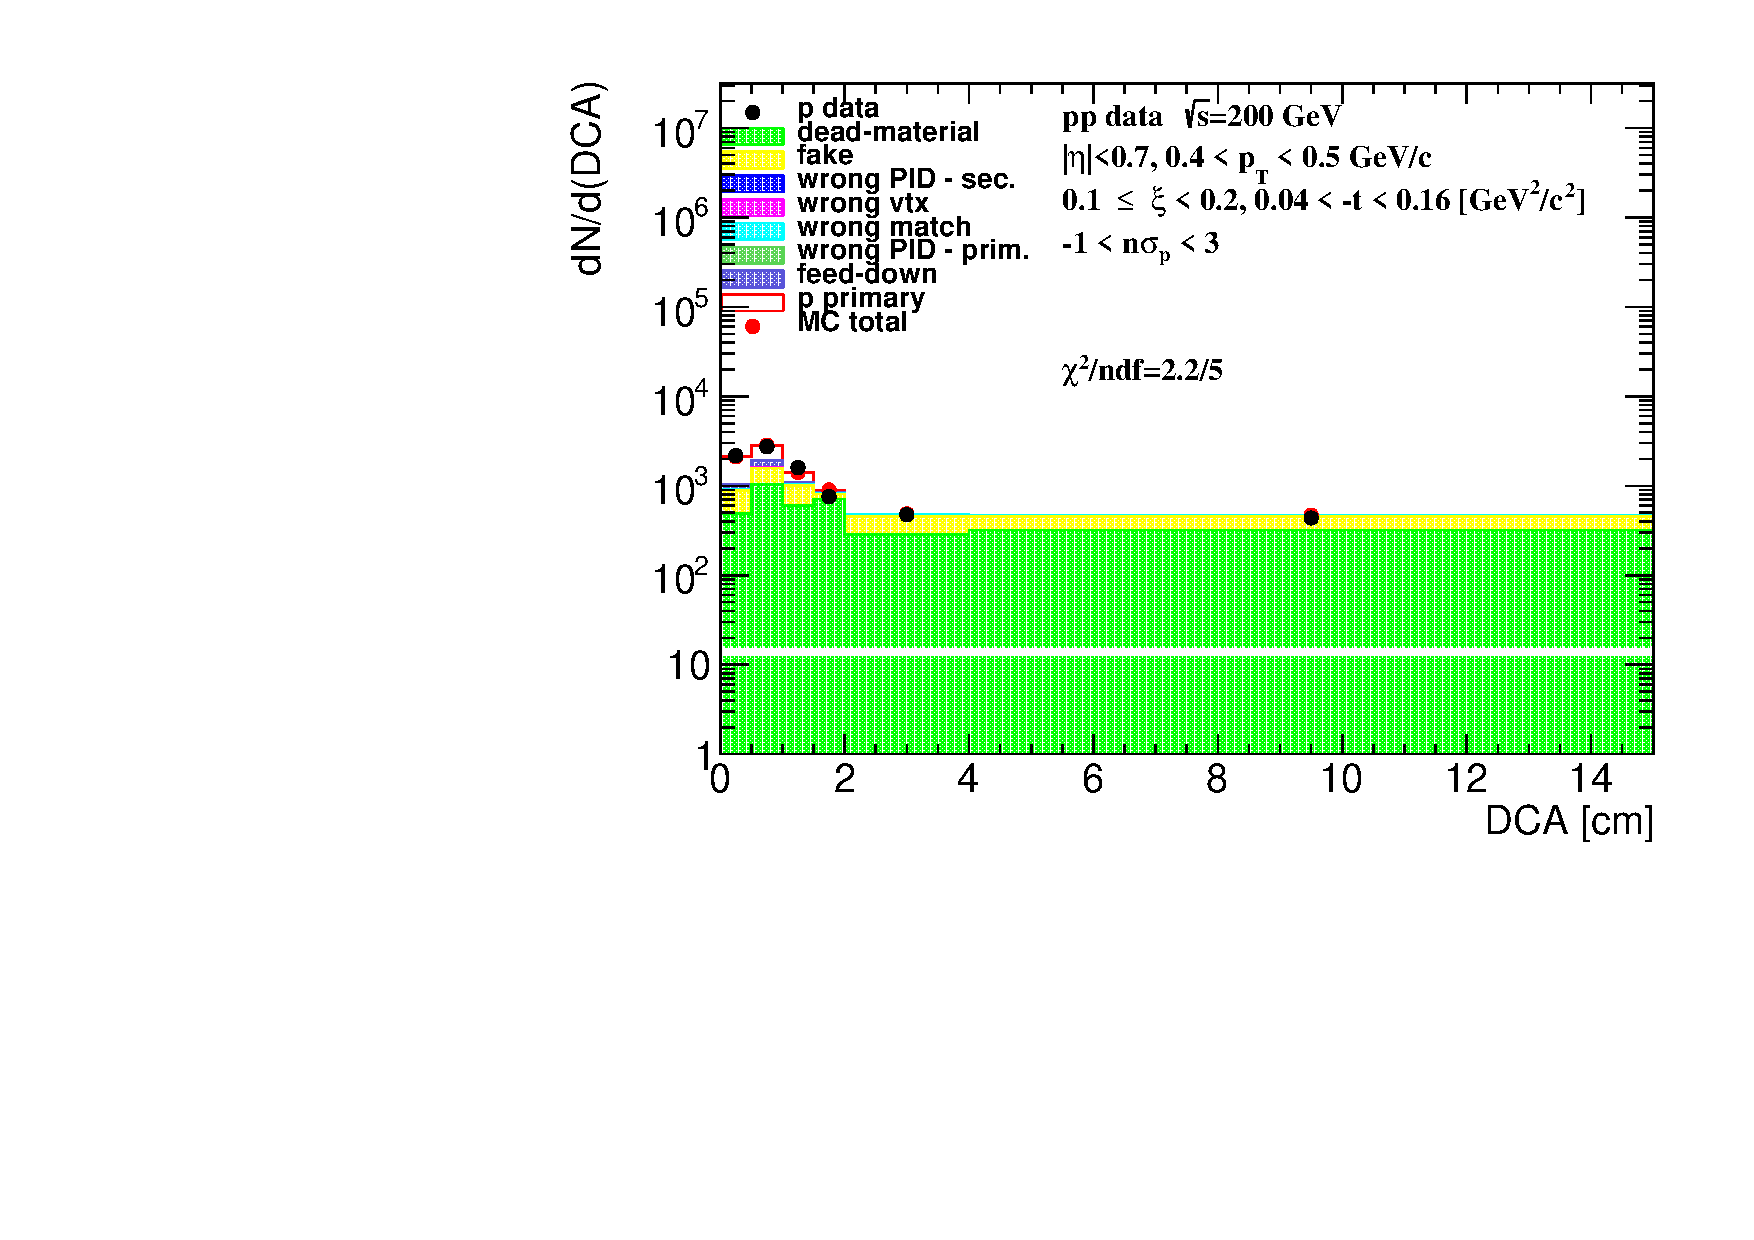
\includegraphics[width=\linewidth, page=1]{chapters/chrgSTAR/img/DCAproton/background_p_2.pdf}
	\end{subfigure}
	\begin{subfigure}{.45\textwidth}
		\includegraphics[width=\linewidth, page=2]{chapters/chrgSTAR/img/DCAproton/background_p_2.pdf}
	\end{subfigure}
	\begin{subfigure}{.45\textwidth}
		\includegraphics[width=\linewidth, page=5]{chapters/chrgSTAR/img/DCAproton/background_p_2.pdf}
	\end{subfigure}
	\begin{subfigure}{.45\textwidth}
		\includegraphics[width=\linewidth, page=6]{chapters/chrgSTAR/img/DCAproton/background_p_2.pdf}
	\end{subfigure}
	\begin{subfigure}{.45\textwidth}
		\includegraphics[width=\linewidth, page=9]{chapters/chrgSTAR/img/DCAproton/background_p_2.pdf}
	\end{subfigure}
	\begin{subfigure}{.45\textwidth}
		\includegraphics[width=\linewidth, page=10]{chapters/chrgSTAR/img/DCAproton/background_p_2.pdf}
	\end{subfigure}
	\begin{subfigure}{.45\textwidth}
		\includegraphics[width=\linewidth, page=13]{chapters/chrgSTAR/img/DCAproton/background_p_2.pdf}
	\end{subfigure}
	\begin{subfigure}{.45\textwidth}
		\includegraphics[width=\linewidth, page=14]{chapters/chrgSTAR/img/DCAproton/background_p_2.pdf}
	\end{subfigure}
	\caption{Distributions of DCA for protons in SD interactions with $0.1 < \xi<0.2$ and loose selection.}
	\label{fig:dca_proton_2}
\end{figure}
\begin{figure}[h!]
	\centering
	\begin{subfigure}{.45\textwidth}
		\includegraphics[width=\linewidth, page=3]{chapters/chrgSTAR/img/DCAproton/background_p_2.pdf}
	\end{subfigure}
	\begin{subfigure}{.45\textwidth}
		\includegraphics[width=\linewidth, page=4]{chapters/chrgSTAR/img/DCAproton/background_p_2.pdf}
	\end{subfigure}
	\begin{subfigure}{.45\textwidth}
		\includegraphics[width=\linewidth, page=7]{chapters/chrgSTAR/img/DCAproton/background_p_2.pdf}
	\end{subfigure}
	\begin{subfigure}{.45\textwidth}
		\includegraphics[width=\linewidth, page=8]{chapters/chrgSTAR/img/DCAproton/background_p_2.pdf}
	\end{subfigure}
	\begin{subfigure}{.45\textwidth}
		\includegraphics[width=\linewidth, page=11]{chapters/chrgSTAR/img/DCAproton/background_p_2.pdf}
	\end{subfigure}
	\begin{subfigure}{.45\textwidth}
		\includegraphics[width=\linewidth, page=12]{chapters/chrgSTAR/img/DCAproton/background_p_2.pdf}
	\end{subfigure}
	\begin{subfigure}{.45\textwidth}
		\includegraphics[width=\linewidth, page=15]{chapters/chrgSTAR/img/DCAproton/background_p_2.pdf}
	\end{subfigure}
	\begin{subfigure}{.45\textwidth}
		\includegraphics[width=\linewidth, page=16]{chapters/chrgSTAR/img/DCAproton/background_p_2.pdf}
	\end{subfigure}
	\caption{Distributions of DCA for protons in SD interactions with $0.1< \xi<0.2$ and normal selection.}
	\label{fig:dca_proton_2t}
\end{figure}
\begin{figure}[h!]
	\centering
	\begin{subfigure}{.45\textwidth}
		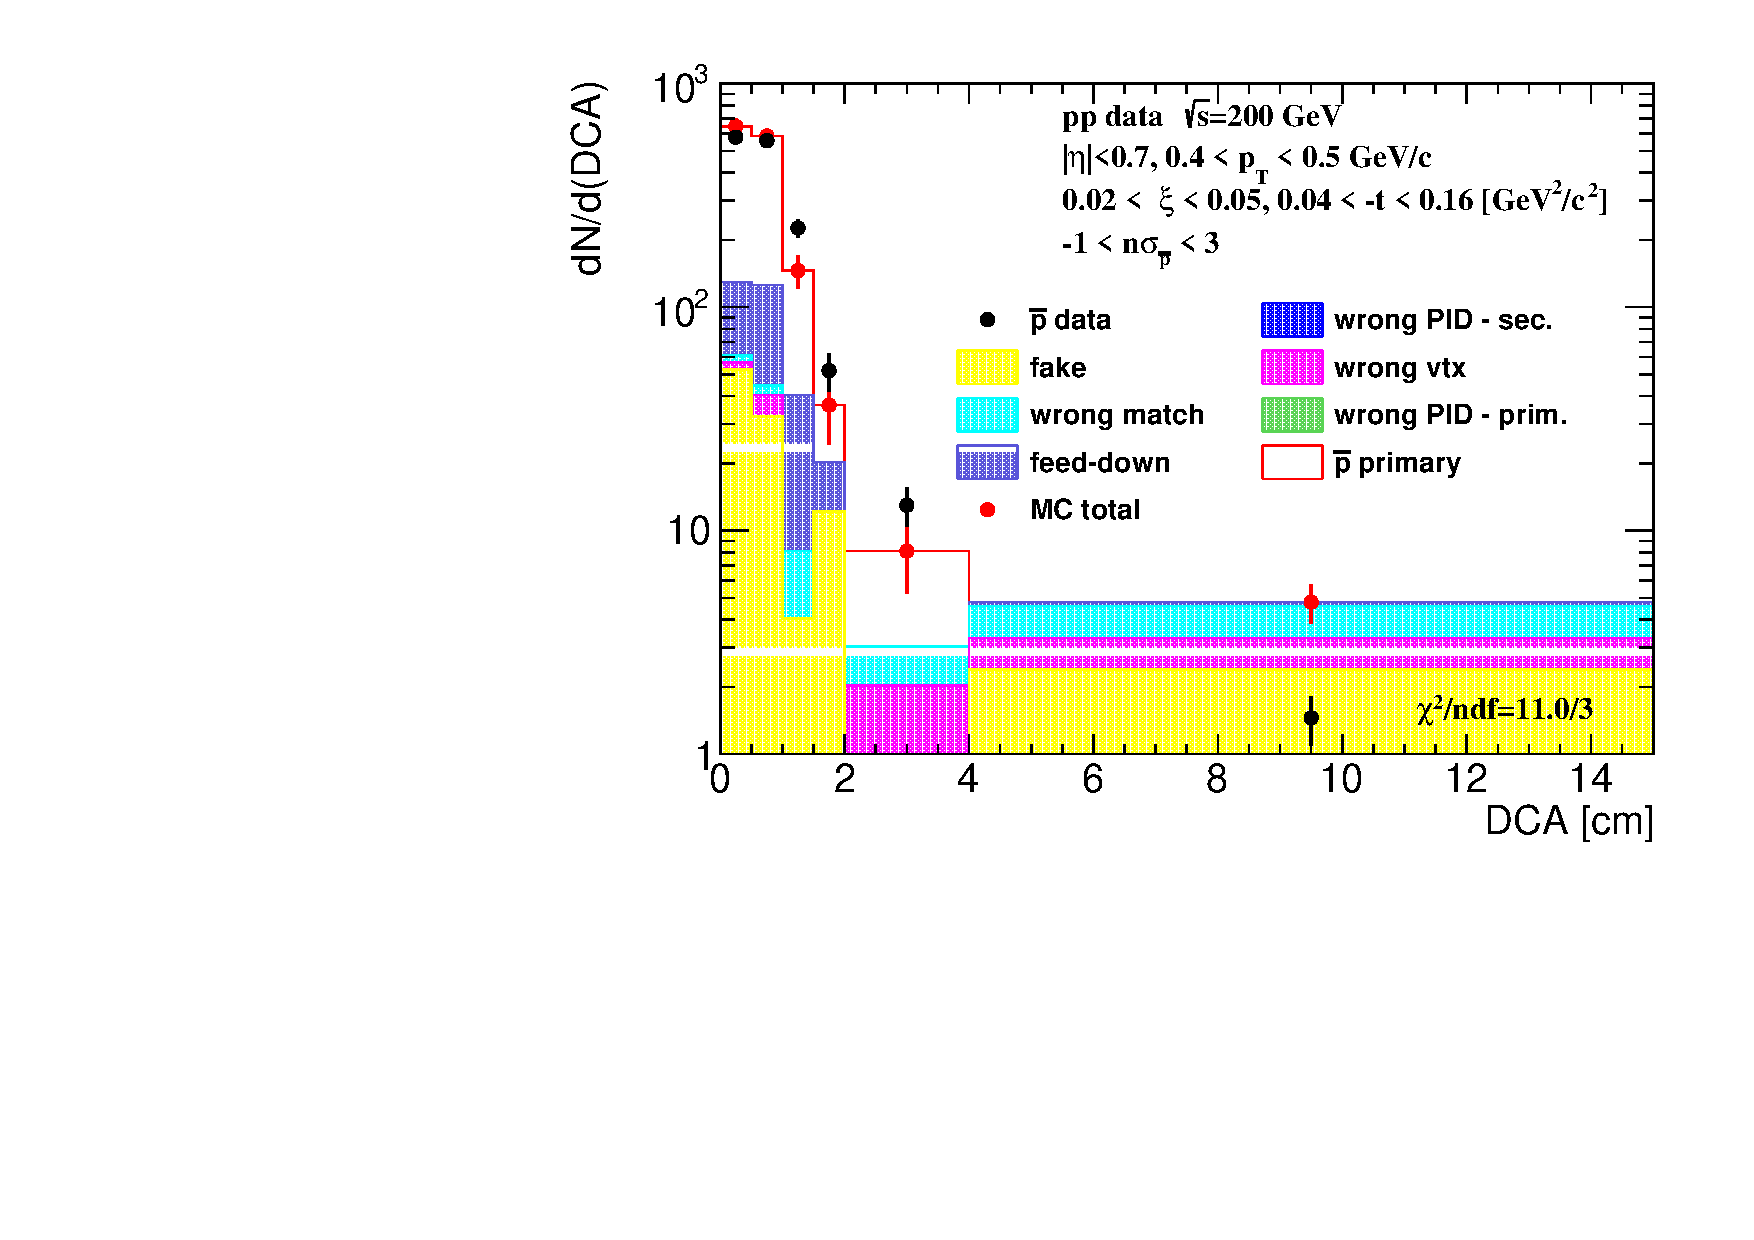
\includegraphics[width=\linewidth, page=1]{chapters/chrgSTAR/img/DCAproton/background_p_bar_0.pdf}
	\end{subfigure}
	\begin{subfigure}{.45\textwidth}
		\includegraphics[width=\linewidth, page=2]{chapters/chrgSTAR/img/DCAproton/background_p_bar_0.pdf}
	\end{subfigure}
	\begin{subfigure}{.45\textwidth}
		\includegraphics[width=\linewidth, page=5]{chapters/chrgSTAR/img/DCAproton/background_p_bar_0.pdf}
	\end{subfigure}
	\begin{subfigure}{.45\textwidth}
		\includegraphics[width=\linewidth, page=6]{chapters/chrgSTAR/img/DCAproton/background_p_bar_0.pdf}
	\end{subfigure}
	\begin{subfigure}{.45\textwidth}
		\includegraphics[width=\linewidth, page=9]{chapters/chrgSTAR/img/DCAproton/background_p_bar_0.pdf}
	\end{subfigure}
	\begin{subfigure}{.45\textwidth}
		\includegraphics[width=\linewidth, page=10]{chapters/chrgSTAR/img/DCAproton/background_p_bar_0.pdf}
	\end{subfigure}
	\begin{subfigure}{.45\textwidth}
		\includegraphics[width=\linewidth, page=13]{chapters/chrgSTAR/img/DCAproton/background_p_bar_0.pdf}
	\end{subfigure}
	\begin{subfigure}{.45\textwidth}
		\includegraphics[width=\linewidth, page=14]{chapters/chrgSTAR/img/DCAproton/background_p_bar_0.pdf}
	\end{subfigure}
	\caption{Distributions of DCA for antiprotons in SD interactions with $0.02 < \xi<0.05$ and loose selection.}
	\label{fig:dca_proton_bar_0}
\end{figure}
\begin{figure}[h!]
	\centering
	\begin{subfigure}{.45\textwidth}
		\includegraphics[width=\linewidth, page=3]{chapters/chrgSTAR/img/DCAproton/background_p_bar_0.pdf}
	\end{subfigure}
	\begin{subfigure}{.45\textwidth}
		\includegraphics[width=\linewidth, page=4]{chapters/chrgSTAR/img/DCAproton/background_p_bar_0.pdf}
	\end{subfigure}
	\begin{subfigure}{.45\textwidth}
		\includegraphics[width=\linewidth, page=7]{chapters/chrgSTAR/img/DCAproton/background_p_bar_0.pdf}
	\end{subfigure}
	\begin{subfigure}{.45\textwidth}
		\includegraphics[width=\linewidth, page=8]{chapters/chrgSTAR/img/DCAproton/background_p_bar_0.pdf}
	\end{subfigure}
	\begin{subfigure}{.45\textwidth}
		\includegraphics[width=\linewidth, page=11]{chapters/chrgSTAR/img/DCAproton/background_p_bar_0.pdf}
	\end{subfigure}
	\begin{subfigure}{.45\textwidth}
		\includegraphics[width=\linewidth, page=12]{chapters/chrgSTAR/img/DCAproton/background_p_bar_0.pdf}
	\end{subfigure}
	\begin{subfigure}{.45\textwidth}
		\includegraphics[width=\linewidth, page=15]{chapters/chrgSTAR/img/DCAproton/background_p_bar_0.pdf}
	\end{subfigure}
	\begin{subfigure}{.45\textwidth}
		\includegraphics[width=\linewidth, page=16]{chapters/chrgSTAR/img/DCAproton/background_p_bar_0.pdf}
	\end{subfigure}
	\caption{Distributions of DCA for antiprotons in SD interactions with $0.02 < \xi<0.05$ and normal selection.}
	\label{fig:dca_proton_bar_t}
\end{figure}
\begin{figure}[h!]
	\centering
	\begin{subfigure}{.45\textwidth}
		\includegraphics[width=\linewidth, page=1]{chapters/chrgSTAR/img/DCAproton/background_p_bar_1.pdf}
	\end{subfigure}
	\begin{subfigure}{.45\textwidth}
		\includegraphics[width=\linewidth, page=2]{chapters/chrgSTAR/img/DCAproton/background_p_bar_1.pdf}
	\end{subfigure}
	\begin{subfigure}{.45\textwidth}
		\includegraphics[width=\linewidth, page=5]{chapters/chrgSTAR/img/DCAproton/background_p_bar_1.pdf}
	\end{subfigure}
	\begin{subfigure}{.45\textwidth}
		\includegraphics[width=\linewidth, page=6]{chapters/chrgSTAR/img/DCAproton/background_p_bar_1.pdf}
	\end{subfigure}
	\begin{subfigure}{.45\textwidth}
		\includegraphics[width=\linewidth, page=9]{chapters/chrgSTAR/img/DCAproton/background_p_bar_1.pdf}
	\end{subfigure}
	\begin{subfigure}{.45\textwidth}
		\includegraphics[width=\linewidth, page=10]{chapters/chrgSTAR/img/DCAproton/background_p_bar_1.pdf}
	\end{subfigure}
	\begin{subfigure}{.45\textwidth}
		\includegraphics[width=\linewidth, page=13]{chapters/chrgSTAR/img/DCAproton/background_p_bar_1.pdf}
	\end{subfigure}
	\begin{subfigure}{.45\textwidth}
		\includegraphics[width=\linewidth, page=14]{chapters/chrgSTAR/img/DCAproton/background_p_bar_1.pdf}
	\end{subfigure}
	\caption{Distributions of DCA for antiprotons in SD interactions with $0.05 < \xi<0.1$ and loose selection.}
	\label{fig:dca_proton_bar_1}
\end{figure}
\begin{figure}[h!]
	\centering
	\begin{subfigure}{.45\textwidth}
		\includegraphics[width=\linewidth, page=3]{chapters/chrgSTAR/img/DCAproton/background_p_bar_1.pdf}
	\end{subfigure}
	\begin{subfigure}{.45\textwidth}
		\includegraphics[width=\linewidth, page=4]{chapters/chrgSTAR/img/DCAproton/background_p_bar_1.pdf}
	\end{subfigure}
	\begin{subfigure}{.45\textwidth}
		\includegraphics[width=\linewidth, page=7]{chapters/chrgSTAR/img/DCAproton/background_p_bar_1.pdf}
	\end{subfigure}
	\begin{subfigure}{.45\textwidth}
		\includegraphics[width=\linewidth, page=8]{chapters/chrgSTAR/img/DCAproton/background_p_bar_1.pdf}
	\end{subfigure}
	\begin{subfigure}{.45\textwidth}
		\includegraphics[width=\linewidth, page=11]{chapters/chrgSTAR/img/DCAproton/background_p_bar_1.pdf}
	\end{subfigure}
	\begin{subfigure}{.45\textwidth}
		\includegraphics[width=\linewidth, page=12]{chapters/chrgSTAR/img/DCAproton/background_p_bar_1.pdf}
	\end{subfigure}
	\begin{subfigure}{.45\textwidth}
		\includegraphics[width=\linewidth, page=15]{chapters/chrgSTAR/img/DCAproton/background_p_bar_1.pdf}
	\end{subfigure}
	\begin{subfigure}{.45\textwidth}
		\includegraphics[width=\linewidth, page=16]{chapters/chrgSTAR/img/DCAproton/background_p_bar_1.pdf}
	\end{subfigure}
	\caption{Distributions of DCA for antiprotons in SD interactions with $0.05 < \xi<0.1$ and normal selection.}
	\label{fig:dca_proton_bar_1t}
\end{figure}
\begin{figure}[h!]
	\centering
	\begin{subfigure}{.45\textwidth}
		\includegraphics[width=\linewidth, page=1]{chapters/chrgSTAR/img/DCAproton/background_p_bar_2.pdf}
	\end{subfigure}
	\begin{subfigure}{.45\textwidth}
		\includegraphics[width=\linewidth, page=2]{chapters/chrgSTAR/img/DCAproton/background_p_bar_2.pdf}
	\end{subfigure}
	\begin{subfigure}{.45\textwidth}
		\includegraphics[width=\linewidth, page=5]{chapters/chrgSTAR/img/DCAproton/background_p_bar_2.pdf}
	\end{subfigure}
	\begin{subfigure}{.45\textwidth}
		\includegraphics[width=\linewidth, page=6]{chapters/chrgSTAR/img/DCAproton/background_p_bar_2.pdf}
	\end{subfigure}
	\begin{subfigure}{.45\textwidth}
		\includegraphics[width=\linewidth, page=9]{chapters/chrgSTAR/img/DCAproton/background_p_bar_2.pdf}
	\end{subfigure}
	\begin{subfigure}{.45\textwidth}
		\includegraphics[width=\linewidth, page=10]{chapters/chrgSTAR/img/DCAproton/background_p_bar_2.pdf}
	\end{subfigure}
	\begin{subfigure}{.45\textwidth}
		\includegraphics[width=\linewidth, page=13]{chapters/chrgSTAR/img/DCAproton/background_p_bar_2.pdf}
	\end{subfigure}
	\begin{subfigure}{.45\textwidth}
		\includegraphics[width=\linewidth, page=14]{chapters/chrgSTAR/img/DCAproton/background_p_bar_2.pdf}
	\end{subfigure}
	\caption{Distributions of DCA for antiprotons in SD interactions with $0.1 < \xi<0.2$ and loose selection.}
	\label{fig:dca_proton_bar_2}
\end{figure}
\begin{figure}[h!]
	\centering
	\begin{subfigure}{.45\textwidth}
		\includegraphics[width=\linewidth, page=3]{chapters/chrgSTAR/img/DCAproton/background_p_bar_2.pdf}
	\end{subfigure}
	\begin{subfigure}{.45\textwidth}
		\includegraphics[width=\linewidth, page=4]{chapters/chrgSTAR/img/DCAproton/background_p_bar_2.pdf}
	\end{subfigure}
	\begin{subfigure}{.45\textwidth}
		\includegraphics[width=\linewidth, page=7]{chapters/chrgSTAR/img/DCAproton/background_p_bar_2.pdf}
	\end{subfigure}
	\begin{subfigure}{.45\textwidth}
		\includegraphics[width=\linewidth, page=8]{chapters/chrgSTAR/img/DCAproton/background_p_bar_2.pdf}
	\end{subfigure}
	\begin{subfigure}{.45\textwidth}
		\includegraphics[width=\linewidth, page=11]{chapters/chrgSTAR/img/DCAproton/background_p_bar_2.pdf}
	\end{subfigure}
	\begin{subfigure}{.45\textwidth}
		\includegraphics[width=\linewidth, page=12]{chapters/chrgSTAR/img/DCAproton/background_p_bar_2.pdf}
	\end{subfigure}
	\begin{subfigure}{.45\textwidth}
		\includegraphics[width=\linewidth, page=15]{chapters/chrgSTAR/img/DCAproton/background_p_bar_2.pdf}
	\end{subfigure}
	\begin{subfigure}{.45\textwidth}
		\includegraphics[width=\linewidth, page=16]{chapters/chrgSTAR/img/DCAproton/background_p_bar_2.pdf}
	\end{subfigure}
	\caption{Distributions of DCA for antiprotons in SD interactions with $0.1 < \xi<0.2$ and normal selection.}
	\label{fig:dca_proton_bar_2t}
\end{figure}